\section{Dynamic Array}

In this section, we will consider the data structure known as dynamic array. It is similar to a regular array, but its length changes according to the ``fullness'' of the array.

\index{dynamic array}

The array will be initialized with a fixed length. Upon calling \textsc{Insert}, it will insert an element into the array, and whenver the current array becomes full, we create a longer array and copy everything into the new array. Similarly, after calling \textsc{Delete}, we will shrink the array whenever the array becomes too empty. If we only consider the worst case, the runtime complexities are bad: $O(n)$ for both operations. However, if we look at the amortized cost, the runtime is actually smaller.

\begin{figure}[htbp]
    \captionsetup{singlelinecheck=false, font=footnotesize, labelsep=space, margin={0pt,1cm}, justification=raggedright}
    \includegraphics[width=0.4\linewidth]{figures/dynamic_arr_append.pdf}

    \hfill

    \caption[width=0.5\linewidth]{The dynamic array after the operation \textsc{Insert}(9). The length of the new array is doubled, and old elements are copied to the new array.}
\end{figure}

\textit{Idea}: When we want to append but the array is full, then we copy the list to an array that is twice as large.

Let $n = \text{\# of elements in the list before an \proc{Append} operation}$. The worst-case cost of \proc{Append} is $n+1$.

\section{Amortized Analysis of Dynamic Array Using Accounting Method}
Let the allocated charge of \proc{Append} be \$3:
\begin{itemize}
    \item \$1 to pay for the write into current array
    \item \$1 to save as credit to pay for itself being copied into a new array
    \item \$1 tax (to pay for a senior citizen to be copied to a new array)
\end{itemize}

Credit invariant: Each element in the last half of the array has \$2 credits.

\begin{proof}
    Base case: No elements in the list. The array size can be 0, 1, or 2. For the first append, the credit invariant is true regardless of the initial size of the array.

    Inductive step: For any future \proc{Append}, assume that the credit invariant is true before it is performed.

    Case 1: If the array is not full, write the element in the first available slot. Use \$1 to pay for the write, and store the remaining \$1. In this case, the credit invariant is clearly maintained after the \proc{Append} operation.

    Case 2: If the array is full, all elements in the last half of the array have \$2 credits (if array size is 1, all elements have \$2). The number of elements in the last half of the array is equal to the number of elements in the first half (or no element in the first half if the array size if 0). Copy the array elements from old array to new array of twice the size. Pay for this using stored \$1 credit. Finally, write the new element to the first available slot. It is the only element in the last half of the new array. Hence, the credit invariant is true.

    By induction, the credit invariant holds.

    Hence, the allocated charge (amortized cost) of \proc{Append} is $\$3 \in O(1)$.
\end{proof}

\begin{figure}[htbp]
    \centering
    \includegraphics[width=0.6\linewidth]{figures/accounting_method_insert.pdf}
    \caption{The credit scheme for amortized analysis of dynamic array.}
    \label{fig:dyarr-amortized}
\end{figure}

\section{Amortized Analysis of Dynamic Array Using Potential Method}

The potential function in any configuration $C$ is defined as
$$
\Phi(C) = (2 \times \text{\# of element in array}) - \text{size of array}
$$
If $C_0$ is the initial configuration and $a_0 \in \{0,1,2\}$ is the initial size of the array, then
$$
\Phi(C_0) = 0 - a_0 = -a_0
$$
Immediately after the first \proc{Append}, $\Phi(C_1) = 2 - \begin{cases} 1 & \text{if $a_0 = 0,1$} \\ 2 & \text{if $a_0 = 2$} \end{cases}$. So $0 \leq \Phi(C_1) \leq 1$.

The amortized cost of the first append with respect to $\Phi$ is
$$
\underbrace{1}_{\substack{\text{actual cost of} \\ \text{writing new element}}} + \begin{cases} 1 \\ 2 \end{cases} \leq 3
$$

Immediately before any subsequent expansion, the number of elements in the array is equal to the size of the array so $\Phi(D)$ is equal to the number of elements in the array.

Immediately after an expansion, $2 \times \text{elements in array} = \text{size of array}$, so $\Phi(D')=0$. So the change in potential can be used to pay for copying elements from old array to new array.

Excluding expansion, an \proc{Append} costs \$1 to write plus \$2 for increase in potential since the number of elements in the array increases one and the size of array does not change).

\section{Deletion From Dynamic Array}

Suppose we also want to allow deletion from the end of the array. A simple algorithm would be: when an array overflows, double it; when an array is less than half full, halve it.

The problem with this algorithm is that the amortized complexity is very big! Consider the following sequence of $n = 2^k + 1$ operations.

\begin{codebox}
    \li \proc{Append} $2^{k-1}+1$ times
    \li \Repeat
        \li \proc{Delete} 2 items
        \li \proc{Append} 2 items \End
    \li $2^{k-3}$ times
\end{codebox}

The time complexity can be summarized as this table

\begin{center}
    \begin{tabular}{c|c|c|c}
        Operations & Number of resulting elements & Size of resulting array & Cost of operations \\
        \hline
        $2^{k-1}-1$ \proc{Append}s & $2^{k-1}+1$ & $2^k$ & $3(2^{k-1}+1)$ \\
        $2$ \proc{Delete}s & $2^{k-1}-1$ & $2^{k-1}$ & $2^{k-1}$ \\
        $2$ \proc{Append}s & $2^{k-1}+1$ & $2^{k}$ & $2^{k-1}+2$
    \end{tabular}
\end{center}

An improved algorithm is: when an array overflows, double it; when an array is less than \textbf{1/4 full}, then halve it.

\subsection{Amortized Analysis of Dynamic Array With Deletion}

Allocated charge for \proc{Append} is \$3 and for \proc{Delete} is \$2. We maintain the following credit invariant:

In a nonempty array of size $2^k$ where $k \geq 0$, there are at least $\lfloor 2^k/4 \rfloor$ elements. Elements in the last half (i.e. last $\lfloor 2^k/2 \rfloor$ slots) have \$2 stored with them. Empty slots in the first half (i.e. first $\lfloor 2^k/4 \rfloor$ slots) have \$1 stored with them.

Prove the credit invariant by induction.

\begin{proof}

    \hfill

    \textbf{Base case}: $k=0$, array is empty. 
    
    \textbf{Inductive step}: Assume the credit invariant is true before some operation. If the array is empty, then the operation must be \proc{Append}.

    If the array is empty, the operation must be \proc{Append}. The element is put into the first half of an array of size 2. There are no elements in the second half and there is no empty slots in the first half. The actual cost of the operation uses \$1. The allocated cost is \$3, so the remaining \$2 can be donated to charity.

    Otherwise, there are four major cases:

    Case 1: Append without overflow:

    Case 1a (append without overflow, with previous expansion): \$1 actual cost, \$2 to store in the data structure.

    \includegraphics[width=0.5\linewidth]{dynamicarr/dynamicarr-case1a.pdf}

    Case 1b (append without overflow, without prior expansion): \$1 actual cost, \$1 from data structure, leftover \$3 can be donated to charity.
    
    \includegraphics[width=0.5\linewidth]{dynamicarr/dynamicarr-case1b.pdf}

    Case 2: Append with overflow: $2^k$ in data structure. Actual cost $2^k+1$. Put \$2 into new array with new element. Allocated charge if \$3 is sufficient.

    \includegraphics[width=0.5\linewidth]{dynamicarr/dynamicarr-case2.pdf}

    Case 3: Delete without contraction

    Case 3a: \$1 actual cost, \$2 in data structure. Leftover \$3 donated to charity.

    \includegraphics[width=0.5\linewidth]{dynamicarr/dynamicarr-case3a.pdf}

    Case 3b: \$1 actual cost, store \$1 in data structure. Allocated charge \$2 is sufficient.

    \includegraphics[width=0.5\linewidth]{dynamicarr/dynamicarr-case3b.pdf}

    Case 4: Delete with contraction: there is \$$2^{k-2}$ in the data structure, which is used to copy elements from old array. \$2 allocated charge donated to charity if there is leftover.

    \includegraphics[width=0.5\linewidth]{dynamicarr/dynamicarr-case4.pdf}
\end{proof}

Since credit invariant is true and the credit in the data structure is at least 0. The amortized cost of \proc{Append} is at most \$3, and the amortized cost for \proc{Delete} is at most \$2.

\section{Amortized Analysis of Dynamic Array With Delete Using Potential Method}

Let $\Phi$ be the potential function such that
$$
\Phi(D) = | 2 \times \text{\# of elements in the list} - \text{size of array} |
$$
Let $D_i$ be the state of the data structure after $i$th operation, and let $c_i$ be the actual cost of the $i$th operation. Let $a_i = c_i + \Phi(D_i) - Phi(D_{i-1})$. If $\Phi(D_n) > \Phi(D_0)$, then $\sum_{i=1}^n a_i = \Phi(D_n) - \Phi(D_0) + \sum_{i=1}^n c_i \geq \sum_{i=1}^{n} c_i$.

The absolute value in the definition of the potential function is necessary because otherwise, the potential in the case of deletion with contraction would be negative.

Let $\Phi(D_0) = 3$. 

Consider the following cases:

\begin{enumerate}
    \item Append without overflow: If elements in the list increases by 1, size of the array does not change, so $\Delta\Phi = \Phi(D_i)-\Phi(D{i-1}) = 2$. Actual cost is 1, so $a_i = 1+\Delta\Phi = 3$.
    \item Append with overflow: $a_i = 2^k + 1 + (2-2^k) = 3$:
    \begin{center}
        \begin{tabular}{c|c|c|}
             & Before & After \\
            \hline
            number of elements & $2^k$ & $2^k + 1$ \\
            array size & $2^{k}$ & $2^{k+1}$ \\
            $\Phi$ & $2^{k}$ & 2   
        \end{tabular}
    \end{center}
    \item Delete without contraction: The number of elements in the list decreases by 1, and array size is unchanged. So, $\Delta\Phi = \Phi(D_i) - \Phi(D_{i-1}) \leq 2$. The actual cost is 1, so $a_i = 1 + \Delta\Phi \leq 3$.
    \item Delete with contraction: The actual cost is $2^k - 1$ so $a_i = 2^k - 1 + 2 - 2^{k+1} \leq 3$:
    \begin{center}
        \begin{tabular}{c|c|c|}
             & Before & After \\
            \hline
            number of elements & $2^k$ & $2^k - 1$ \\
            array size & $2^{k+1}$ & $2^{k+1}$ \\
            $\Phi$ & $2^{k+1}$ & 2   
        \end{tabular}
    \end{center}
\end{enumerate}

In all cases, $a_i \geq 3$, so the amortized cost of \proc{Append} and \proc{Delete} is at most 3.